\section{Proposta}

Este estudo propõe o desenvolvimento de um protótipo voltado para a geração procedural de mapas que incorporam biomas, sendo o contorno determinado a partir de dois cenários distintos: uma representação gráfica de um desenho e uma fotografia do cotidiano.

Na imagem do desenho, a utilização de uma técnica de segmentação para a detecção de objetos será empregada, contribuindo para a seleção do contorno. Por sua vez, na fotografia do cotidiano, será adotado um modelo de segmentação panóptica. Este modelo, conforme delineado na \cref{fig:etapas_proposta}, processará a imagem, proporcionando ao usuário a possibilidade de escolher o contorno desejado. O resultado final replicará o contorno da seleção em ambas as dimensões, bidimensional e tridimensional.

A \cref{fig:etapas_proposta} esboça os passos a serem seguidos para uma imagem urbana, onde a imagem de entrada (a) representa o ponto de partida do processo de segmentação panóptica e o resultado (imagem b) é obtido mediante o emprego do modelo EfficientPS, desenvolvido por Mohan et al. (2020). Este modelo, reconhecido por sua eficiência e elevada qualidade na classificação panóptica de pessoas, torna-se crucial em contextos urbanos contemporâneos. Após a segmentação, o usuário tem a capacidade de selecionar o contorno por meio de técnicas de escolha de cor e preenchimento de inundação, conforme detalhado por OpenCVInRange e OpenCVFloodFill, respectivamente.

O desfecho nos dois cenários — fotografia do cotidiano e desenho — é uma máscara binária, isolando o objeto na imagem, como evidenciado na imagem c, que destaca a escolha do segmento, tal como o carro amarelo na imagem b.

Posteriormente, um mapa procedural será gerado com o contorno selecionado, conforme exemplificado na imagem d. Essa representação incluirá uma sobreposição do contorno do veículo, meramente para ilustrar que a ilha gerada terá um contorno semelhante. As cores na representação indicam o oceano (azul), a floresta (verde) e as montanhas (cinza), seguindo a classificação de biomas.

Após essas etapas, a atualização automatizada do relevo do mapa tridimensional será realizada. Adicionalmente, será incorporada uma visualização conjunta do mapa em 3D e 2D no Unity, sendo o mapa 3D jogável e o 2D funcionando como minimapa, oferecendo uma noção de localização no contexto tridimensional (Amit, 2010; First Person Movement). Testes com métricas de segmentação serão conduzidos para avaliar a similaridade entre a entrada da geração procedural e a saída, validando a hipótese de que uma maior densidade de pontos no diagrama de Voronoi resultará em maior precisão nos contornos das imagens.

\begin{figure}[!ht]
	\centering
    \caption{Etapas da proposta}
	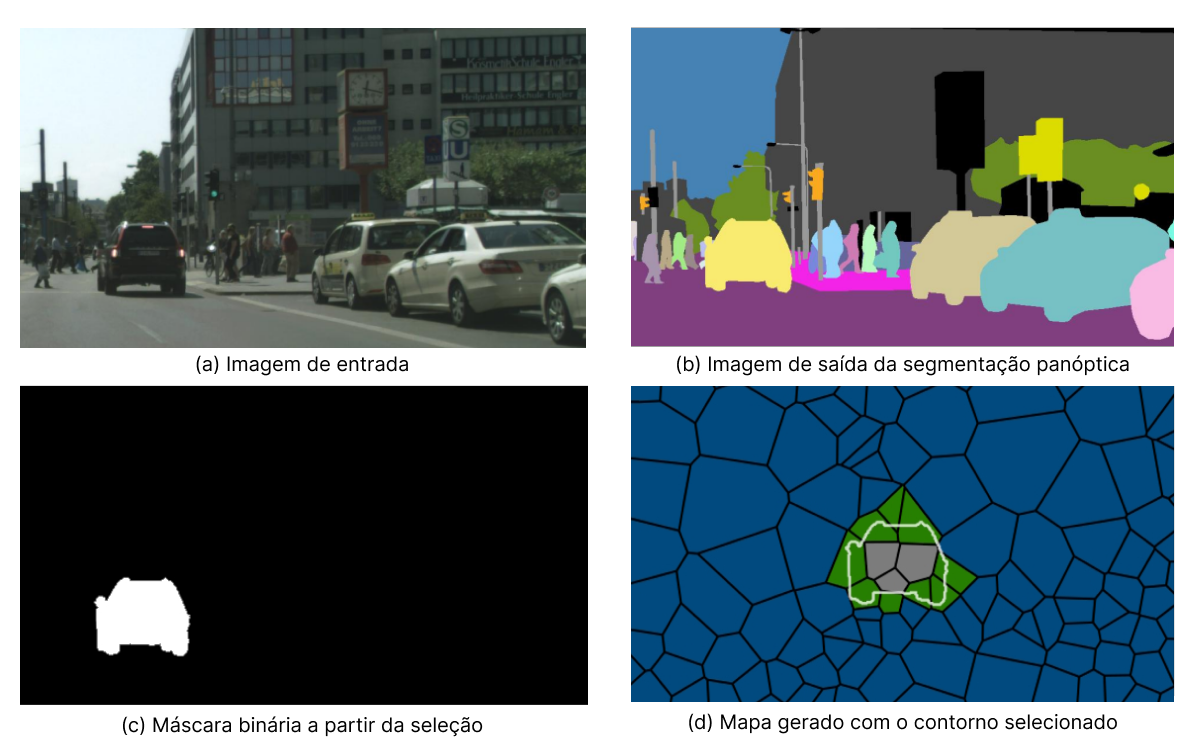
\includegraphics[width=0.9\textwidth]{figures/etapas_proposta.png}
    \legend{Fonte: \citeonline{kirillov2019panoptic} e autoria própria}
	\label{fig:etapas_proposta}
\end{figure}
